\documentclass[preprint,12pt,authoryear]{elsarticle}
\journal{Labour Economics}
\usepackage{geometry}   
\geometry{
	a4paper,
	total={170mm,257mm},
	left=20mm,
	top=20mm,
}
\usepackage{amsmath}
\usepackage{fixmath}
\usepackage{natbib}
\usepackage{comment}
\DeclareMathOperator{\Jac}{J}
\usepackage{float}
\usepackage{graphicx}
\usepackage{caption}
%\usepackage{subfig}
\usepackage{subcaption}
\usepackage{lscape}
\usepackage{booktabs,calc}
\usepackage[usenames, dvipsnames]{color}
\usepackage{color,soul}
\usepackage{authblk}
\newcommand{\ra}[1]{\renewcommand{\arraystretch}{#1}}
\usepackage{threeparttable}
\usepackage{lscape}
\usepackage{adjustbox}
%\usepackage{floatrow}
%\usepackage{amssymb}
\usepackage{verbatim}
\usepackage{pythontex}
\usepackage{dcolumn} 
\usepackage[toc,page]{appendix}
\newcolumntype{d}[1]{D{.}{\cdot}{#1}}  
\usepackage[hidelinks]{hyperref}
\hypersetup{colorlinks=false}
\usepackage{footmisc}
%\renewcommand{\footnotelayout}{\doublespacing}
\usepackage{setspace}
\usepackage{dsfont}
\usepackage{tikz}
\usetikzlibrary{decorations.pathreplacing,arrows.meta}
%\linespread{1.2}


\begin{document}
	
\title{The Task \& Skill Content of Occupational Transitions over the Business Cycle: Evidence for the UK}


\author{Aspasia Bizopoulou \fnref{label4}}
\ead{aspasia.bizopoulou@vatt.fi}
\ead[url]{https://sites.google.com/site/aspasiabizopoulou/home}
\fntext[label4]{Senior Researcher, VATT Research Institute}
\address{Economicum
	
	Arkadiankatu 7
	
	PL 1279, 00101 Helsinki, Finland\fnref{label5}}
%\fntext[label5]{Senior Researcher}

\author{Rachel Forshaw\corref{cor1}\fnref{label2}}
\ead{r.forshaw@hw.ac.uk}
\ead[url]{https://sites.google.com/site/racheljoyforshaw}
\fntext[label2]{Assistant Professor, Heriot-Watt University}
\cortext[cor1]{Corresponding author}
\address{Campus The Avenue, Heriot-Watt University, Edinburgh, EH14 4AS UK\fnref{label3}}

\begin{comment}

		
	\author{Aspasia Bizopoulou\footnote{Senior Researcher, VATT Institute for Economic Research, 7 Arkadiankatu, 00101 Helsinki, Finland\\ email: aspasia.bizopoulou@vatt.fi} $\quad$ Rachel J. Forshaw\footnote{Corresponding Author. Assistant Professor, Heriot-Watt University, Edinburgh, EH14 4AS UK; email: r.forshaw@hw.ac.uk}} 
	\title{\textbf{The Task \& Skill Content of Occupational Transitions over the Business Cycle: Evidence for the UK\footnotetext{\llap{\textsuperscript{}} An earlier version of this paper formed part of our PhD theses, which were funded by University of Edinburgh Research and Teaching Scholarships. We would like to thank Liang Bai, Carlos Carillo-Tudela, Mike Elsby, Julian Fennema, Maia G\"{u}ell, Cristina Lafuente,  Tuomas Pekkarinen, Eva Pocher, Jean-Marc Robin, Mark Schaffer, Anna Salomons, Jonathan Thomas and Ludo Visschers for their helpful comments as well as participants from the RES, SMYE, ESPE, EEA-ESEM, SaM, EALE, SGPE, Economics at Panmure House conferences; from seminars at VATT, ETLA, Aalto University, Edinburgh, the Scottish Government and from the IAB Nuremberg. Any remaining errors are our own. }}}

	%\date{\textbf{Preliminary Draft- please do not distribute}}
	
	
	
	\maketitle
	
	content...
	\end{comment}
	
	\vspace{-5mm}
	
	\begin{abstract}
		
		Using the UK Labour Force Survey matched with O*NET detailed task and skill data for the period \input{../Results/min_date.txt}\hspace{-1mm}-\input{../Results/max_date.txt}\hspace{-1mm}, we present evidence that the change in tasks and skill level in job-to-job transitions is broadly similar within and outside of recessions. These results are in contrast to studies using occupation category as a proxy for occupational content, which have tended to find that the probability of making occupational category changes is strongly pro-cyclical. 

	
	

		
	\end{abstract}

	\textbf{Keywords}: occupational mobility, tasks, skills, business cycles, Double Hurdle, selection. 
	
	\vspace{2mm}
	
	\textbf{JEL Codes}: J62, E32
	
	\newpage
	\doublespacing
	\section{Introduction}
	\label{sec:Introduction}
	
	Periods of increased unemployment entail changes to the reallocation processes of the labour market. In particular,  \cite{Carrillo-Tudela2016},  \cite{MurphyTopel1987}, \cite{Moscarini2007} and \cite{Kambourov2008} document a pro-cyclical relationship in the number of job-to-job transitions both in the UK and the US. Yet, while there many studies documenting how the number of transitions decreases in recessions, comparatively less is known about what happens to the content of those transitions in terms of the tasks and skills undertaken as part of occupations. Previous literature, including \cite{MurphyTopel1987}, \cite{Moscarini2007}, \cite{Kambourov2008}, \cite{Carrillo-Tudela2014}, \cite{Carrillo-Tudela2016}, have used occupational titles as a proxy for the content of occupations, finding occupational transitions to be strongly pro-cyclical. 	
	In this paper, we break down occupational titles to actual job tasks and specific skill levels, and show that this strong pro-cyclical relationship is no longer evident: recessions negatively impact job transitions but have very little impact on individuals' propensity to change their occupational content. 
	
		\vspace{2mm}
	
	Characterising an occupation as a group of separate tasks is a relatively recent but already well-established practice in the literature studying job transitions. Among applied papers, \cite{Poletaev2008} are one of the first to map occupational titles to tasks from the US Dictionary for Occupational Titles. %Using factor analysis, they group the tasks into four major categories and subsequently rank them by the intensity that they are used in each occupation. 
	They study content difference in occupational switchers, defined as the situation when the new occupation employs the previous occupation's main skill with much lower or much higher intensity. They find that wage losses are closely associated with switching skill portfolio, in particular a decrease in skills. The key difference to our study is that their sample is of displaced workers, whereas we focus on all job-to-job transitions. %[add the \cite{Robinson2018 reference too}] 
	In a similar vein, \cite{Gathmann2010} and subsequently \cite{robinson2018} construct a measure of occupational distance based on tasks, which we modify to use in this paper. Using German administrative data, they find that individuals tend to switch to occupations with similar task requirements, and the change in task composition of occupational moves tends to decrease over time.  Pioneered by \cite{ALM2003} and furthered by \cite{AcemogluAutor2011}, \cite{AutorDorn2013}  and \cite{GoosManningSalomons2014}, a large body of literature studies changes in the returns to skills and the evolution of earnings inequality. In particular, this literature categorises tasks as manual or cognitive and finds that labour demand is changing as a result of automation, leading to wage and employment gains for cognitive tasks relative to manual tasks and leading to job polarization. Our work differs from this literature in that it looks at the long-term trends of task change whereas our concern is the variation over the business cycle.
	
	\vspace{2mm}
	

	
	
	
	\vspace{2mm}
	
	
	A separate literature studies job transitions over the business cycle. \cite{Carrillo-Tudela2016} look at the propensity for individuals to change careers over the cycle and find that the probability of a career change co-moves positively with the cycle. In addition, they find that career movers receive higher wages than those who do not change occupations. \cite{Devereux2000} offers an early study of the cyclicality of task assignment, focusing within the firm. He finds that firms tend to re-assign individuals to tasks of lower quality during recessions. \cite{Summerfield2016} shows that recessions lead to an increase in the share of tasks in the economy that are classified as manual. The contribution of the current paper to this literature is to address whether individuals overall tend to move to more or less similar jobs in terms of tasks during recessions, and whether the direction of these moves in terms of the required skill level is affected by economic conditions.
	
	
	


	\vspace{2mm}


\noindent The intuition for why our paper finds results that are contradictory to the literature is twofold.  Firstly, we are able to calculate the combined impact of recessions on both i) the probability of changing tasks at all as measured by an occupational transition (which we will call the \textit{extensive} margin) and ii) the extent of the task change for those undertaking an occupational change (which we will call the \textit{intensive} margin). Using the \cite{Mcdonald1980} decomposition we estimate that \input{../Results/fracMeanPos_angSep_CASCOT_r.txt}\hspace{-1mm}\% of the overall relationship that we estimate is the result of the latter intensive margin, i.e. the part attributable to a change in task or skill content. Previous studies captured only the extensive margin and as such tended to over-estimate the relationship between business cycles and occupational transitions. The second reason for why we find contradictory results is that there is selection in the types of individuals that change occupations in recessions. We use a Double Hurdle model to explicitly capture both the intensive and extensive margins, and allow for correlation in the errors of the two processes. When we control for selection this further reduces the magnitude of the total relationship between business cycles and occupational change.



	
	\vspace{2mm}
	
	In our analysis we focus on the part of the working population that makes employment-to-employment (henceforth E2E) moves, which represents just over 50\% of new hires in the UK. This population of new hires is an important barometer of the labour market's relationship with  business cycles since, adjusting for productivity, the rate of job-to-job transitions is a sufficient statistic for the average real wage in the economy (\cite{MoscariniPostelVinay}). Our analysis requires a way to quantify task and skill changes, leading us to focus the first part of the paper on presenting a suitable measure of change in task composition from the literature which we modify to fit our specific purposes. We also propose a second measure to extract skill level information from the task data. We then detail the Double Hurdle model used to understand the relationship between tasks and skill content of occupational changes and the business cycle. Since the decision to change tasks consists of two parts, namely i) the decision to change tasks at all and ii) how big a task move to make, we decompose the estimates to obtain separate figures for each element. We find that the cyclical nature of task and skill changes is quantitatively small, and when we control for the composition effects of the types of people who get hired in a recession, it is statistically insignificant. 
	
	
	\vspace{2mm}
	
	
 In section \ref{sec:Data} we describe the data that we use. Section \ref{sec:measures} presents the measures of task and skill difference between occupations. Section \ref{sec:Model} describes the econometric models used, and section \ref{sec:results} reports the results. Finally, section \ref{sec:Conclusion} concludes.
	


	
	\section{Data}
	\label{sec:Data}
	We first describe the data on job transitions in section \ref{sec:LFS}, then the data on task and skill content of occupations in section \ref{sec:ONET}. Section \ref{sec:matchLFSONET} describes how we match the two datasets.
	\subsection{UK Labour Force Survey (LFS)}
	\label{sec:LFS}
	
	We use the UK Quarterly Labour Force Surve (LFS) for the years \input{../Results/min_date.txt}\hspace{-1mm}-\input{../Results/max_date.txt}\hspace{-1mm}. We focus on this time period as our data contains a consistent classification of occupations, Standard Occupational Classification (SOC2010) codes throughout the sample, and it spans the 2008-9 recession.\footnote{While occupational classifications are available for the 1990s and 2010s, occupations are classified according to a very different set of criteria. As such, when compared over time it is unclear what is true variation in occupations and what is simply reclassification.}  In the LFS respondents are followed over a maximum of five quarters, and in each quarter a fifth of the sample is replaced by an incoming group. For the majority of our analysis, we focus on individuals over two quarters only.\footnote{With the exception of a robustness check in which we estimate the relationship between skill level and wages in section \ref{sec:wagesSkills}, in we use the 5 quarter longitudinal sample.} The advantage of using the 2 over the 5 quarter sample is that we have a much larger number of observations, on average 30,000 individuals per quarter.\footnote{Over time, the LFS has decreased the number of interviewed individuals. In the early years of our sample, each sample has close to 60,000 individuals, while in the later years it drops to about 20,000 per quarter. All estimations and graphs include population weights so that the decreasing number of respondents doesn't bias the results.} We are able to study job-to-job transitions that do not involve a quarter or more of unemployment or inactivity between employment spells.\footnote{The individual may still experience a small period of unemployment, given the nature of a quarterly survey.} 
	%The survey contains information on individuals' employment status, their employment SOC code, employer tenure, sex, education, reasons for leaving their last job, methods of searching for new jobs, type of work contract (permanent or temporary) and type of employment (employed or self-employed). The series are weighted using census population weights provided by the Office for National Statistics (ONS).
	%\newpage
	
	\subsection{US O*NET}
	\label{sec:ONET}
	
	\begin{figure}[t]
		\centering
		\includegraphics[width=1\linewidth]{../Figures/ONETQn}
		\caption{O*NET Example Question}
		\caption*{\small{Example question concerning mathematical reasoning from the O*NET, source: US O*NET Abilities Questionnaire}}
		\label{fig:ONETQn}
	\end{figure}
	
	\begin{figure}[h]
		\begin{center}
			\includegraphics[scale=0.30]{../Figures/SOC2ONET2.png}
			\caption{Example of mapping the SOC2010 to the O*NET }
			\caption*{\small{The SOC2010 code that covers occupation `Economist' is 2425 and also covers a number of other occupations, including Actuary and Bioinformatician. Code 2425 maps to multiple O*NET occupations. Taking an average over all of the Oral Comprehension scores for the different O*NET occupations gives a score for the SOC2010 code. }}
			\label{fig:SOC2ONET}
		\end{center}
	\end{figure}
	
	
	\begin{figure}[h!]
		\centering
		\includegraphics[width=1\linewidth]{../Figures/ScoreRange}
		\caption{O*NET Task Vector Example - Economist}
		\caption*{\small{Example task vector. The y axis lists all the tasks in occupation 2425 (Economist), the x axis is a normalised score of the skill level required for each task. Black dots are the O*NET exact matches for occupation 2425, red dots are the average values across the different possible matches and constitute the final scores that we use in our analysis for this occupation. Source: author's calculations using US O*NET and CASCOT.}}
		\label{fig:ONETScoreRange}
	\end{figure}
	
	The US Department for Labor's O*NET dataset is a highly detailed survey which provides us with a picture of the tasks that are used in occupations. We standardise occupational classifications available in the LFS to match occupations to the US O*NET. Our aim is to obtain a detailed task content and difficulty profile for each occupation and to subsequently measure the distance between different occupations based on similarity of task content and level of skill. We choose to map the O*NET to UK occupational codes as, while some data about the task content of UK jobs exists in the UK Skills Survey, the O*NET is much more suitable for our purposes.\footnote{The UK Skills Survey contains both labour market variables found in the LFS and task data found in the O*NET, however its sample size is too small for focusing only on job-to-job transitions to run our estimations. For the task data, it would be theoretically possible to average over the observations to get job content for occupations. However, the questions are much more qualitative than the O*NET - variables include `Importance of looking the part' and `how often come home from work exhausted'; which, although interesting in their own right, do not readily map to tasks. It also doesn't cover all occupations because they are not sampled. \cite{ONETreport} use the method employed in this paper to map the O*NET to UK SOC codes. They find the method to be robust, to create useful and reasonable data for occupations, and to accord with Skills Survey data in the variables that feature in both.} 
	
	Alongside task data, the O*NET allows us to recover information on the required skill level at which each task is used in each occupation. We refer to this as `skill level', since the O*NET gives us information about both the type of task in the occupation and the level at which it is performed. To illustrate, figure \ref{fig:ONETQn} shows the question asked for the job task `mathematical reasoning'. The skill level score ranges from 1 to 7. In this particular example, a skill level of 1 corresponds to ``Determine how much 10 oranges will cost when they are priced at 2 for 20 cents'', and a score of 6 corresponds to ``Determine the mathematics required to simulate a spacecraft landing on the moon'', the latter being clearly higher skilled. In section \ref{sec:taskDistance}, below, we show the measures used to ascertain the difference between two occupations and to separate out task and skill information. 
	
	\subsection{Matching the O*NET task data to the UK LFS}
\label{sec:matchLFSONET}

	
A crucial element in this study is the ability to match UK SOC codes from the LFS with task information from the O*NET. To do this we utilise CASCOT (Computer-Assisted Structured Coding Tool), a software tool developed by the Warwick Institute For Employment Research.\footnote{More information available at https://warwick.ac.uk/fac/soc/ier/software/cascot/} CASCOT is a computer program designed to make a semantic match between occupational titles and standard occupational codes. This mapping is created by comparing text descriptions of UK SOC2010 occupations to text descriptions of O*NET occupations.
	
	The O*NET contains task profiles for 974 occupations, which we map onto the 374 SOC2010 occupations of the UK LFS using the CASCOT software. Since the number of separate occupation categories in the US are almost 3 times as many as the number of occupational categories in the UK Standard Occupational Classification that is used in the LFS, the mapping is not one-to-one, but one-to-many. In order to get a single task vector for each UK SOC code, we follow two steps: first we use a confidence-weighted average over all matching O*NET occupations, where the confidence weights for the mapping of O*NET codes to UK SOC codes are provided by the CASCOT software.\footnote{We use a confidence threshold of 70\%, dropping any matches that fall below this confidence level. A visual inspection of the mapping confirms that the matches are sensible.} We obtain a mapping similar to the one shown in Figure \ref{fig:SOC2ONET}, where SOC code 2425 (left panel) is mapped with 6 different O*NET codes (right panel). Each O*NET occupation has scores for each of the 147 tasks in terms of the level of skill needed to perform a job. In this example, we look at the task `oral comprehension'. In figure \ref{fig:SOC2ONET} SOC code 2425 that covers occupation `Economist' is mapped with several possible occupations from the O*NET, including `Actuary' and `Statistician'. Taking an average over all of the oral comprehension scores for the different O*NET matches gives a single score for this task in the SOC2010 code, which we then repeat for all possible tasks in all possible matches. Figure \ref{fig:ONETScoreRange} provides an illustration of the average score for every task that is part of an Economist's portfolio, as calculated in Figure \ref{fig:SOC2ONET}.
	
	

	
	\section{Capturing content changes across occupations}
	\label{sec:measures}
	We first detail our measure of tasks in section \ref{sec:taskDistance}, then our measure of skills in section \ref{sec:changeSkillLevel}. Section \ref{sec:twoTaskEx} shows a simplified example of the two measures and section \ref{sec:wagesSkills} establishes that higher skill level is associated with higher wages in the data. Finally, section \ref{sec:advantageTasks} discusses why it is important to incorporate these measures of tasks and skills when considering occupational changes.
	\subsection{Measuring the Change in Tasks}
	\label{sec:taskDistance}
	To measure the change in task composition between two occupations we use the measure of angular separation from \cite{Gathmann2010}, which has also been used in the innovation literature (\cite{Jaffe1986}). The measure of the change in task composition between two occupations is as follows:
	
	
	\begin{equation}
	\label{eq:angSep}
	\Delta \text{Tasks}_{o,o'} = \left(1 - \frac{\sum_{t=1}^{T}(q_{t,o}\times q_{t,o'})}{\left[(\sum_{t=1}^{T}q_{t,o}^{2})\times(\sum_{t=1}^{T}q_{t,o'}^{2})\right]^{\frac{1}{2}}}\right)   \in [0,1]
	\end{equation}
	
	\noindent where $o,o'$ is a pair of different occupations, $t$ is tasks, $q_{t,o}$ represents the skill level of a task $t$ within occupation $o$. Intuitively, the change in task composition between a set of occupations $o$ and $o'$ are compared by measuring the angle between their respective vectors. The scores in the vectors range between 0 (this task is not used in an occupation) and 7 (this task is used at the highest level), which we normalise within $[0,1]$, so that the entire measure is within $[0,1]$. Each occupation is represented by a vector of equal length dimension and each element of the vector gives a task score, i.e. the intensity with which the task is used in the given occupation. Some of the elements of the vector are zeros, since occupations do not use all available tasks. 
	The way we apply equation \ref{eq:angSep} is different to the usage by \cite{Gathmann2010}, in which they use data on the fraction of employees using task $t$ in occupation $o$ to comprise $q_{t,o}$. Their data only carries information about the composition of tasks, rather than the skill level, whereas our task vectors include both. Therefore we develop another measure, detailed below in section \ref{sec:changeSkillLevel} which captures the difference in skill level between task vectors.
	
	
	
	\begin{comment}
	\begin{figure}[H]
	\centering
	\begin{minipage}{.4\textwidth}
	\centering
	\begin{tabular}{lc} %\toprule
	&\input{../Figures/angSep_diff_quantile.txt} \\
	%\bottomrule	
	\end{tabular}
	\end{minipage}
	\begin{minipage}{.4\textwidth}
	\centering
	\begin{tabular}{lc} %\toprule	
	&\input{../Figures/angSep_same_quantile.txt} \\
	%\bottomrule	
	\end{tabular}
	\end{minipage}
	\caption{Quantiles of task similarity of potential occupational moves across (left) and within (right) 1-digit SOC codes (including zeros)}
	\label{fig:angSep_quantile}
	\end{figure}
	\end{comment}
	
	\subsection{Measuring the Change in Skills}
	\label{sec:changeSkillLevel}
	In our dataset, since the length of the vector for each occupation is determined by the difficulty - or skill level - at which the tasks is required, by measuring its length we can capture the degree of upskilling or downskilling between occupations. We propose the following measure, which takes into account the differences in magnitude between two vectors, to capture the change in skill level: 
	
	\begin{equation}
	\label{eq:skillScore}
	\Delta\text{Skills}_{o,o'} = \left[\left[\sum_{t=1}^{T}(q_{t,o'}^{2})\right]^{\frac{1}{2}} - \left[\sum_{t=1}^{T}(q_{t,o}^{2})\right]^{\frac{1}{2}} \right]/\sqrt{T} \in[-1,1]
	\end{equation}
	
	
	\noindent Equation \ref{eq:skillScore} calculates the difference in length of two occupation task vectors and has range $[-1,1]$; -1 means that moving occupations results in complete downskilling in every task, 0 means two occupations are equally skilled in every task, 1 complete upskilling in every task.\footnote{Theoretically, a value of 0 could mean that the two vectors do not have the exact same scores for each task but the differences happen to offset each other perfectly. However, we do not observe this in the data - i.e., no two pairs of different SOC codes return a value of exactly 0. } The measure is therefore symmetric, i.e. $\Delta\text{Skills}_{{A}{B}}  = -1* \Delta\text{Skills}_{{B}{A}}$.
	
		\subsection{Two-Task Example of the Task and Skill Change Measures}
	\label{sec:twoTaskEx}
	
	Figure \ref{fig:AngSep} provides an illustration of how the $\Delta$Task and $\Delta$Skills measures can provide us with information about the content of occupational moves. We construct a basic example in which there are a total of four different occupations ($A$, $B$, $C$, $D$) which comprise two tasks: task 1 and task 2. Moving from occupation $A$, which is highly skilled in task 1 and task 2, to $B$, which is lowly skilled in both tasks gives a change in task composition of 0, since the tasks are still used in the same proportion. The $\Delta$Skills$_{o,o'}$ of $\input{../Figures/AB_skillScore.txt}$ reflects the fact that occupation $B$ is much lower skilled than $A$. Moving from occupation $C$ to $A$ represents both a change in tasks and upskilling, whereas the change in tasks from $A$ to $D$ constitutes downskilling. Finally, moving from and to the same occupation $A$ results in zeros for both measures.
	
	\begin{figure}[h]
		\centering
		\includegraphics[scale=0.60]{../Figures/AngularSeparation_example}
		\qquad
		\begin{tabular}{lcc}
			Occupation move & $\Delta$Tasks$ _{o,o'}$& $\Delta$Skills$_{o,o'}$\\
			\hline
			\hline
			A $\rightarrow$ B & 0 & \input{../Figures/AB_skillScore.txt}  \\
			C $\rightarrow$ A &  \input{../Figures/CA_angSep.txt} & \input{../Figures/CA_skillScore.txt}  \\
			A $\rightarrow$ D &  \input{../Figures/AD_angSep.txt} & \input{../Figures/AD_skillScore.txt}  \\
			A $\rightarrow$ A & 0 & 0 \\
		\end{tabular}
		\caption{An example of $\Delta$Tasks and $\Delta$Skills with 2 tasks and 5 occupations}
		\label{fig:AngSep}
	\end{figure}
	
	\subsection{The Relationship between Skill Level and Wages}
	\label{sec:wagesSkills}
	In using the $\Delta$Skills measure, equation \ref{eq:skillScore}, we are assuming that vector length of occupations is a good proxy for skill level of the tasks completed in an occupation. If the measure is capturing skill level we should expect it to be positively correlated with wages. To test this assumption we calculate the skill level for each occupation in the LFS: \\
	
	 Skill Level$_{o}$ = $\left[\sum_{t=1}^{T}(q_{t,o}^{2})\right]^{\frac{1}{2}} $ \\
	 
	\noindent  i.e. it is a measure of the vector length of an occupation in the task space, or the left hand side of the term in brackets of equation \ref{eq:skillScore}. We use this measure in a standard Mincerian wage estimation: 
	\begin{equation}
	\label{eq:skill_returns}
	\ln w_{it}= \alpha + \beta_{1}\text{ Skill Level}_{o}+  \sum_{k} \beta_{k}X_{k,it} + e_{it}, 
	\end{equation}
	
	where $\ln w_{it}$ are log real gross weekly wages for individual $i$ at time $t$. The vector $X_{it}$ includes controls for age, age squared, a dummy equal to 1 for female, years of tenure in the current job and dummies for high, medium and low eduction. Skill Level is standardised by subtracting its mean and dividing by its standard deviation to facilitate interpretation. We use the five quarter LFS and take the wage to be the one seen in the last quarter of interview. The sample includes all types of job histories ending with employment in the fifth quarter of interview.
	
	\vspace{2mm}
	
	The estimation of Equation \ref{eq:skill_returns} can been seen in table \ref{skill_returns}. A one standard deviation increase in skill level is associated with an increase of \input{../Results/beta_SkillTotal.txt}\hspace{-1mm}\% in weekly gross real wages. This result suggests that our measure of the length of the vector as a skill difficulty proxy is reasonable since it is strongly positively correlated with wages. 
	
	
	\begin{table}[t]
		\centering
		\begin{tabular}{l*{1}{c}}
			\input{../Results/returns_skill_2000s}
		\end{tabular}
		\caption{Estimated Returns to Skills} 
		\caption*{\footnotesize Notes: Dependent variable is log real gross weekly wages. Esimated on the LFS 5Q sample of full time workers using wages observed in the first interview quarter. Skill Level is proxied by linked O*NET data and standardised. The coeficient on Age$^2$ is multiplied by 1000. The reference category for education is Low Education (no qualifications). Standard errors in parentheses;	* \(p<0.10\), ** \(p<0.05\), *** \(p<0.01\)}
		\label{skill_returns}
	\end{table}
	
	
	

	
	\subsection{The Advantage of Using Task Data}
	\label{sec:advantageTasks}
	Before proceeding to apply the above measure in our analysis, we take a moment to highlight the advantage of using task data to characterise how the content of two occupations might be different. In mobility studies, authors usually use highly aggregated occupational codes, as in \cite{Carrillo-Tudela2016} who use 1-digit SOC codes, \cite{kambourov2009occupational} who use 1- and 2- digit occupational codes in the PSID. We argue that such aggregated measures seem to capture very little of the content difference between two occupations. This can be seen anecdotally by looking at the occupation titles across different 1-digit occupations which can be more similar than transitions within the same 1-digit occupation. For example, moving from being a `Manager, food and beverage' employee (5436) to working in `Textiles, garments and related trades' (5419) would not be recorded as a change according to the 1-digit SOC definition of content change whereas the move to `Manager, public house' (1224) would. 
	
	\vspace{2mm}
	
	Formalising this observation, figure \ref{fig:angSep_diff} shows the distributions of all potential within- and across-1 digit SOC code occupation moves that can be made in terms of the change in task composition (equation \ref{eq:angSep}). We calculate the change in task composition of every occupation pair and plot the score in the left distribution if the first digit of the occupation code differs (an `across' 1-digit occupation move, which is the type of move usually recorded as a `content' change in the literature) or the right hand distribution if the first digit of the occupation code is the same (a `within' 1-digit move, which is not captured as a change in content when using 1-digit SOC codes). If SOC codes capture differences in task content well we should expect the across-distribution (left) to have measures of central tendency to the right of those of the within-SOC (right) code distribution, which would reflect a notion of a large occupational move or `career change' when making across-code moves. However, while larger moves are slightly more likely in the across-code (left) distribution, we see that the two distributions are remarkably similar. 
	
	\begin{figure}[H]
		\centering
		\begin{minipage}{.5\textwidth}
			\centering
			\includegraphics[width=1\linewidth]{../Figures/all_angSep_diff1Digit_nonzero}
		\end{minipage}%
		\begin{minipage}{.5\textwidth}
			\centering
			\includegraphics[width=1\linewidth]{../Figures/all_angSep_same1Digit_nonzero}
		\end{minipage}%
		\caption{Task distance of potential occupational moves across (left) and within (right) 1-digit SOC codes (excluding zeros)}
		\label{fig:angSep_diff}
	\end{figure}
	
	
	\begin{table}[H]
		\centering
		\input{../Figures/angSep_diff_same_quantile.tex} 
		%\bottomrule	
		\caption{Quantiles of task similarity of potential occupational moves across (left) and within (right) 1-digit SOC codes (including zeros)}
		\label{fig:angSep_quantile_diff_same}
	\end{table}
	
	
	
	
	




 \section{Methodology}
\label{sec:Model}

We use three different specifications to estimate the relationship between the economic cycle and tasks and skills. The first, in section \ref{sec:4digit},  is closest to existing literature. Whereas this literature models the intensive decision of whether there is an occupational change, our econometric specification also captures the extensive decision of whether there is a task change by using a Tobit specification on 4-digit occupational code data.

Our use of task data necessitates a more granular measure of occupational change: we use 4-digit occupational codes rather than the 1-digit codes commonly employed in the literature. As such, in section \ref{sec:1digit}  checks the robustness of our results by aggregating the 4-digit codes to 1-digit categories.

Finally, in section \ref{sec:selection} we address the concern of selection effects, given that the types of people that change jobs in a recession are likely different to the types of people that change jobs outside of a recession. 


\subsection{4-digit Occupational Level}
\label{sec:4digit}
Our first specification is outlined below in Equation \ref{eqn:tobit}. This regression specification is similar to that of \cite{Carrillo-Tudela2016}, however where they estimate a Probit, we use a Tobit model. We do this because our measures of change in task composition and change in skill level are not binary, but continuous on $[0,1)$. A large portion of the sample (approximately 40\%) is censored at zero. Individuals censored at zero are those who experience a job transition, but don't change their occupation code. Individuals that do not change codes may still change tasks since even the most detailed 4-digit SOC codes aggregate occupations into groups, as was shown in section \ref{sec:ONET}. Hence the data is censored, and so a Tobit is the appropriate specification. Below we summarise the model:

\begin{equation}
\label{eqn:tobit}
y_{it,2} =\max(0,\beta_0 + \beta_{1}u_{t} + \sum_{j} \beta_{j}X_{j,it,12} + \sum_{k} \alpha_{k} \text{Q}_{k,1} + \sum_{l} \gamma_{l} \text{R}_{l,1} + \sum_{m} \delta_{m} \text{I}_{m,1}+ e_{it})
\end{equation}

\noindent Here, $i$ represents individuals; $t$ is time; $j$ are individual-level and job-level controls, $Q$ are quarters, $R$ regions, $I$ industries; $e_{it}$ is the error term. $y_{it}$ is the dependent variable, which is either $\Delta\text{\textit{Tasks}}_{it}$ when estimating the relationship between the cycle and the change in task composition of moves or $|\Delta\text{\textit{Skills}}_{it}|$ when estimating the relationship between the cycle and the absolute change in skill level. We take the absolute value of the change in skill level since we cannot have an upper and lower truncation limit for the Tobit equal to zero (as this would imply no truncated values). A subscript of $,\hspace{-0.5mm}1$ or $,\hspace{-0.5mm}2$ designates whether the data is taken from the first quarter that a respondent is interviewed, second quarter, and $,\hspace{-0.5mm}12$ denotes both.

\vspace{2mm}

Our independent variable of interest is $u_{t}$, i.e. the aggregate unemployment rate. We add a set of controls wch include demographic characteristics, namely age and age squared, marital status, sex, level of education.\footnote{We split education into low, medium and high. In the low category we only include individuals with no qualifications; in the middle we include those with at least an Entry Level Qualification and at most A levels (a UK pre-requisite for university entry); and in the high we include all those with any qualification above A levels.} We also add a set of variables related to the individual's current and previous job: the duration of the previous employment and whether the separation was voluntary/involuntary or related to retirement, as well as controls for whether either job is temporary, part- or full-time, self-employed, and in the public or private sector. Finally, we have a set of controls for the method by which the individual searches for new jobs: through a job centre, ads, direct applications, family/friends, or some other method. The rest of the controls are a set of dummies marking quarters to control for seasonality as well as a set of regional dummies to capture regional differences within the UK.

\subsubsection{1-digit Occupational Level}
\label{sec:1digit}

Our second specification addresses the concern that our use of 4-digit occupation codes may obscure the phenomenon that we are investigating. Previous literature has used much more aggregated 1- or 2-digit occupational codes to look at this question, which make occupational change in general less likely, and large occupational changes more likely. To illustrate this point, we graph the probability of occupation change, as defined in \cite{Carrillo-Tudela2016}, in which the probability of career change at the k-digit (k=1,2,3,4) is estimated as:

\begin{equation*}
\text{Prob Career Change$^{k}$ = } \frac{E2E^{k}_m}{E2E^{k}_s + E2E^{k}_m}
\end{equation*}

\noindent where $E2E^{k}_m$ is the number of individuals that changed jobs and moved k-digit occupation; and $E2E^{k}_s$ is the number of individuals that changed jobs and did not move their k-digit occupation. For example, an Economist is in occupational code 2 at the one-digit level. If she changed occupations to become a Florist (SOC 5 at the one-digit level), this would be classed in the numerator as an E2E move. If, however, she became a management consultant (occupational code 2), this would be classed in the denominator as a one-digit stay.


\begin{figure}[h]
	\centering
	\includegraphics[width=1.0\linewidth]{../Figures/prob_career_change}
	\caption{Probability of Career Change at 1-,2-,3- and 4-digit Occupation Codes}
	\caption*{\small{Five quarter moving average of the probability of career change as estimated as the ratio of E2E movers that changed a) 1-digit, b) 2-digit, c) 3-digit, d) 4-digit occupation to those E2E that stayed within the respective occupational digit.}}
	\label{fig:probCareerChange}
\end{figure}

To make our analysis as comparable to previous results as possible, we also estimate equation \ref{eqn:tobit} with dependent variables  $\Delta\text{\textit{Tasks}}_{i}$ and $|\Delta\text{\textit{Skills}}_{i}|$ aggregated to the 1-digit occupational code level. To do so, we calculate the average potential task or skill move from all 4-digit occupational codes with first digit $j$ to all 4-digit occupational codes with first digit $k$ to be the task or skill change for any moves between $j\hspace{-1mm}\star\hspace{-1mm}\star\star$ and $k\hspace{-1mm}\star\hspace{-1mm}\star\star$. Moves from 4-digit code $j\hspace{-1mm}\star\hspace{-1mm}\star\star$ to the same first digit $j\hspace{-1mm}\star\hspace{-1mm}\star\star$ will have task and skill distance zero. For example, a move from 1121 to 2462 has the same task distance, 0.07 (the average task change of all possible moves from occupations with first digit 1 to first digit 2), as a move from 1221 to 2444.

\subsection{Selection Concerns and Double Hurdle Estimation}
\label{sec:selection}

One issue that arises in the estimation of equation \ref{eqn:tobit}  is the possibility of selection bias. Our population of interest consists of individuals undertaking a job-to-job transition. Since the volume of job transitions decreases in recessions, the composition of those who make a job-to-job transition in a recession is likely different to those who do so in normal economic conditions. Table \ref{tab:diffMeans} confirms there are significant differences in observable characteristics between the recession and and non-recession samples. Those that make a job-to-job transition in a recession are older, more likely to be married and have longer tenure. Fewer are in temporary roles for their previous or current job, and a larger fraction are self employed or work for the public sector in either their previous or current job. More are high-educated and a lower fraction are medium- or low- educated. Fewer have quit (made a voluntary separation) from their previous employer, and a larger fraction have been fired (made an involuntary separation).  


\begin{table}[h]
	\centering
	\caption{Difference in Means of E2E Sample In and Outside Recession}\label{tab:diffMeans}
	\begin{adjustbox}{max width=16cm, max height=11cm}
		\begin{threeparttable}
			\input{../Results/t_test.tex}
			\begin{tablenotes}
				\item \footnotesize{Notes: Difference in longitudinal-weighted means inside=1 and outside=0 of recession for E2E movers in the LFS 2Q sample. Recession periods defined using UK ECRI indicator. Significance levels:$ \quad ^{*}<10\% \quad ^{**}<5\% \quad ^{***}<1\%$. Standard errors in parentheses. Source: author's calculations.}  
			\end{tablenotes}
		\end{threeparttable}
	\end{adjustbox}
\end{table}


\begin{figure}
	\begin{center}
		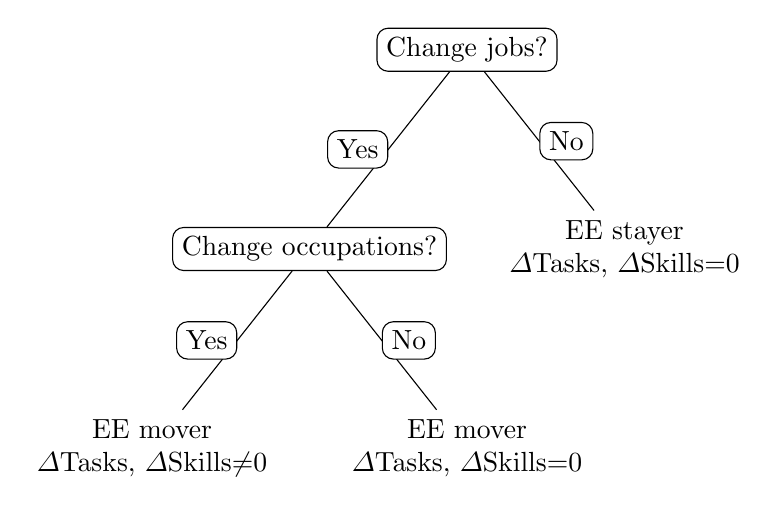
\begin{tikzpicture}[sibling distance=4cm,
		every node/.style = {shape=rectangle, rounded corners,
			draw, align=center,
			top color=white}]]
		\tikzset{level distance=72pt}
		\node {Change jobs?}
		child {node {Change occupations?} child {node[draw=none,fill=none]{EE mover\\$\Delta$Tasks, $\Delta$Skills$\neq$0} edge from parent node[left] {Yes}} child {node[draw=none,fill=none]{EE mover \\ $\Delta$Tasks, $\Delta$Skills=0} edge from parent node[right] {No}} edge from parent node[left] {Yes}}
		child {node[draw=none,fill=none]{EE stayer \\ $\Delta$Tasks, $\Delta$Skills=0} edge from parent node[right] {No}};
		\end{tikzpicture}
		\begin{tikzpicture}
		\draw [decorate,decoration={brace,amplitude=10pt},xshift=-4pt,yshift=0pt] (3.5,7.5) -- (3.5,4.65) node [black,midway,xshift=35pt,text width=1.5cm] {\footnotesize  Selection};
		\draw [decorate,decoration={brace,amplitude=10pt},xshift=-4pt,yshift=0pt] (3.5,4.5) -- (3.5,1.65) node [black,midway,xshift=35pt] {\footnotesize Censoring};
		\end{tikzpicture}
	\end{center}
	\caption{Illustration of Double Hurdle model} \label{fig:flowE2E}
	\caption*{\small{First step: whether an individual changes jobs. Second step: whether an individual changes occupations (whether they have a task and skill change.)}}
\end{figure}


While we control for these observable composition changes in our estimations, a question remains about whether this selected sample will bias estimates if there is remaining unobserved heterogeneity. To explore this, we adopt a third regression specification using a Double Hurdle model proposed by \cite{cragg1971}, and applied in a labour market setting by \cite{BlundellMeghir} and \cite{Blundell1989}. This bivariate model captures the intensive and extensive margins of recessions on job transitions, illustrated in figure \ref{fig:flowE2E}. The first hurdle, is a Probit model, capturing whether an individual decides to change jobs or not. If they do not change jobs, their $\Delta$ Tasks and $\Delta$ Skills will be always be zero. In the second hurdle, if the individual has changed jobs, they must decide whether to change occupations. If they change occupations, $\Delta$ Tasks and $\Delta$ Skills will be non-zero. If they do not change occupations, their $\Delta$ Tasks and $\Delta$ Skills will appear as zero in the data. Note though, there is the same censoring issue as discussed in section \ref{sec:4digit} - they may change tasks and skills but not occupation codes -  so for this second step a Tobit model is also the correct specification. Concretely, the equations of the Double Hurdle model are:


\begin{subequations}
	\label{eqn:heckman}
	\begin{align}
	& EE_{it,2} = \tilde{\beta}_0 + \tilde{\beta}_{1}\text{Available}_{t,1} + \sum_{j} \tilde{\beta}_{j}\hat{X}_{j,it,1} + \sum_{k} \tilde{\alpha}_{k} \text{Q}_{k,1} + \sum_{l} \tilde{\gamma}_{l} \text{R}_{l,1} + \sum_{m} \tilde{\delta}_{m} \text{I}_{m,1}+  \tilde{e}_{it} \label{eqn:heckmanProbit}\\
	& y_{it,2}^{**} = \check{\beta}_0 + \check{\beta}_{1}u_{t} + \sum_{j} \check{\beta}_{j}X_{j,it,12} + \sum_{k}\check{\alpha}_{k} \text{Q}_{k,1} + \sum_{l} \check{\gamma}_{l} \text{R}_{l,1} + \sum_{m} \check{\delta}_{m} \text{I}_{m,1}+ \hat{\lambda}_t + \check{e}_{it} \label{eqn:heckmanTobit_start} \\
	& y_{it,2}^* =\max(0, y_{it,2}^{**})  \label{eqn:heckmanTobit_end} \\
	& y_{it,2} = EE_{it,2}y_{it,2}^* \label{eqn:dh} 
	\end{align}
\end{subequations}


Equation \ref{eqn:heckmanProbit} is the Probit selection model which has dependent variable $EE$ equal to one if an individual changes jobs between the first and second quarter of interview, and zero otherwise. Note that control variables $\hat{X}$ differ from those in the structural equation, since we include only first-period controls for characteristics of the respondent's previous job. We also omit search method as only those that changed jobs were asked which search method they used.  Equation \ref{eqn:heckmanTobit_start} and  \ref{eqn:heckmanTobit_end} are the Tobit structural model with dependent variables as in equation \ref{eqn:tobit}, either $\Delta\text{\textit{Tasks}}_{i}$ or $|\Delta\text{\textit{Skills}}_{i}|$. This specification is the same as \ref{eqn:tobit}, with the addition of the estimated inverse Mills ratio obtained from estimating equation \ref{eqn:heckmanProbit}, $\hat{\lambda}$, to control for selection. Equation \ref{eqn:dh} governs the relationship once the hurdle `changed jobs' has been passed.  The Double Hurdle model is similar to the Tobit model of \ref{eqn:tobit}, but allows the extensive and intensive margins to be governed by distinct stochastic processes. That is, unlike the Tobit model, it allows different processes to determine the value of the continuous (non-zero) observations and the discrete switch at zero. This is important for our purposes since there is no reason to expect that the relationship between the unemployment rate and the decision to switch jobs, and the relationship between the unemployment rate and the decision to change tasks or skills, is the same. This modelling approach is also related to the control function advanced by \cite{Heckman}, but whereas the Heckit model assumes first hurdle dominance - ie. that in the second stage there will be no zero observations, the Double Hurdle model allows zero observations to arise. As in a Heckman model, we allow the errors of the first and second hurdles to be correlated. As such, to avoid multicollinearity issues we also include the instrument \textit{Available}, whether the individual is available to start work in the next two weeks. The instrument for the selection equation is a dummy which captures whether an individual is available to start work in the next two weeks. This will be equal to one if the respondent is looking for a new job, is waiting to start a new job or would like a new job but has not yet started searching and would be able to start a job in the next two weeks. This instrument is highly predictive of the dependent variable in the selection equation - whether the individual changed jobs between the first and second quarter of their survey. However, it should not have any bearing on the size of the task or skill change that an individual makes after changing jobs, the dependent variable in the two structural equations. 
	
\section{Results}
\label{sec:results}


%\subsection{Changes in Tasks and  Skills over the Cycle}
%\label{sec:TobitProbit}


To control for the changing composition of E2E transitions over the cycle, we estimate the Tobit model of equation \ref{eqn:tobit}. Results are shown in model (1) of table \ref{tab:TobitResults}. We see that an increase in the unemployment rate of one percentage point is associated with \input{../Results/angSep_sd_CASCOT.txt}\hspace{-1mm} of a standard deviation reduction in task change.\footnote{\input{../Results/agg_urate_angSep_CASCOT.txt}\hspace{-1mm} times the APE factor, \input{../Results/APEfactor_angSep_CASCOT.txt}\hspace{-1mm}} The magnitude of this relationship is very small. To put this into context, we estimate that the conditional average of $\Delta$Task Change is \input{../Results/angSep_s_mean.txt}\hspace{-1mm}\footnote{Conditional on the compositional controls listed in table \ref{tab:TobitResults}.}. An example of a move with $\Delta$Task composition equal to \input{../Results/angSep_s_mean.txt}\hspace{-1mm}  is from $4159$ `Fraud Inspector' to $3533$ `Insurance Underwriter'. During the 2008 recession, the unemployment rate increased by approximately 2.5 percentage points. The estimated standard deviation of $\Delta$Task composition, conditional on the controls listed in section \ref{sec:Model}, is \input{../Results/angSep_s_sd.txt}\hspace{-1mm}. An increase in the unemployment rate by 2.5 percentage points would therefore correspond to an approximate change of:
\[
\underbrace{2.5}_{\Delta Xu}* \underbrace{\input{../Results/agg_urate_modOfMod_ape_CASCOT.txt}}_{\widehat{\frac{\partial E(y| X)}{\partial Xu}}} *\underbrace{\input{../Results/angSep_s_sd.txt}}_{ \widehat{E(\sigma|X)}} = \input{../Results/agg_urate_context.txt}
\]

\noindent In our example, this would be an occupational move with $\Delta$Tasks=\input{../Results/angSep_s_mean.txt}\hspace{-1mm} \input{../Results/agg_urate_context.txt} =  \input{../Results/agg_urate_context2.txt}\hspace{-1.5mm}. An example of such a task move is 3532 `Insurance Broker' to 4132 `Administrative Officer, Insurance'. Both of these examples are small occupational moves, and there seems to be minimal difference between the two types of moves.

\vspace{2mm}

In terms of the absolute change in skill level (i.e. when $y_i=|\Delta\text{\textit{Skills}}_{i}|$), the estimate is in the same direction and of a similar magnitude. An increase in the aggregate unemployment rate corresponds to a \input{../Results/agg_urate_modOfMod_ape_CASCOT.txt} change in skill level.\footnote{\input{../Results/agg_urate_modOfMod_CASCOT.txt} times the APE factor,\input{../Results/APEfactor_modOfMod_CASCOT.txt}\hspace{-1mm}, table \ref{tab:TobitResults}} This estimated relationship is similarly economically insignificant.
\newpage
\newgeometry{a4paper,left=1in,right=1in,top=1in,bottom=1in,nohead}
%\begin{landscape}
\thispagestyle{empty}
\begin{table}[htbp]
	\centering
	\caption{Changes in Tasks and Skills over the Cycle}\label{tab:TobitResults}
	\begin{adjustbox}{width=\textwidth}
		\begin{threeparttable}
			% \input{../Results/tobit_ALL_2000s.tex}
			
			\input{../Results/tobit_ALL_2000s.tex}
			\begin{tablenotes}
				\item{\footnotesize{(1) Tobit at the 4-digit occupation category level. (2) Tobit at the aggregated 1-digit occupation category level (3) Double Hurdle at the 4-digit occupation category level. The sample in the selection equation of specification (3) is all individuals aged 16-64 years old over the period \input{../Results/min_date.txt}\hspace{-1mm}-\input{../Results/max_date.txt}\hspace{-1mm} and employed in both the first and second quarter of their survey. The sample in all other other specifications have the additional restriction that individuals undertook a job transition over two quarters (i.e., changed employers). The coefficient on age squared is multiplied by 1000. The reference category for education is Low Education; for Job Separation it is `Voluntary';  for Job seeking method it is `Not Looking'. The regression includes seasonal, regional and industry fixed effects. Coefficients should be  multiplied by the APE factor where given to obtain correct marginal effect. Standard errors in parentheses.}}
			\end{tablenotes}
		\end{threeparttable}
	\end{adjustbox}
\end{table}
%\end{landscape}
\restoregeometry % Restore the global document page margins
\newpage

\doublespacing

With the addition of task data to occupations, we are able to look not just at the \textit{probability of changing occupations} during recessions but also the \textit{extent of the change} of the task content. \cite{Mcdonald1980} show that the marginal effect of a Tobit model can be decomposed as follows:\footnote{See appendix \ref{app:TobitDecomp} for details}$^{,}$\footnote{Note that, unlike the reported Tobit marginal effects in table \ref{tab:TobitResults}, for ease of interpretation of probabilities this decomposition is not standardised and so it sums to the unstandardised marginal effect, \input{../Results/totalEffect.txt}\hspace{-1mm}.}


\begin{equation}
\resizebox{\columnwidth}{!}{$\displaystyle
	\label{eqn:tobit_decomp}
	\underbrace{\frac{\partial E(y| X)}{\partial Xu}}_{\text{Total marginal effect}} = \underbrace{P(y>0|X)}_{\substack{\text{Probability of changing} \\ \text{ occupations}\\=\input{../Results/APEfactor_angSep_CASCOT_t.txt}}}\times\underbrace{\frac{\partial E(y|X, y>0)}{\partial Xu}}_{\substack{\text{Change in expected task move} \\ \text{given occupation move} \\ \text{following a change in} \\ \text{the unemployment rate} \\ =\input{../Results/dEystarbydXi_angSep_CASCOT.txt}}} + \underbrace{ E(y|X, y>0)}_{\substack{\text{Expected task move} \\ \text{given occupation move}\\=\input{../Results/Eystar_angSep_CASCOT.txt}}}\times \underbrace{\frac{\partial P(y>0|X)}{\partial Xu}}_{\substack{\text{Change in probability of} \\ \text{occupation move}  \\ \text{following a change in} \\ \text{the unemployment rate}\\=\input{../Results/dFzbydXi_angSep_CASCOT.txt}}}
	$}
\end{equation}


\vspace{3mm}
Of particular interest to this study is the relationship between the unemployment rate and the change in task composition given that there is an occupation change, i.e. the term $\frac{\partial E(y|X, y>0)}{\partial X_{u}}$, as opposed to the term $\frac{\partial P(y>0|X)}{\partial X_u}$ which only measures the impact on the probability of changing occupation and has previously been shown to be negative and economically significant. Here, we estimate this change in probability to still be negative, but it is not as large in magnitude as in previous research. This is due to our definition of occupational change being much more granular, at the 4-digit occupational code rather than 1-digit as in previous work.
Using $z \equiv X\beta/\sigma$ and the cumulative normal distribution function $F(z)\equiv P(y>0|X)$ and dividing both sides of equation \ref{eqn:tobit_decomp} by $F(z)\beta_{u}$, we can get the expression:

\begin{equation}
\frac{\partial E(y|X, y>0)}{\partial X_{u}}=\pi_{u}*\beta_{u}
\end{equation}

\noindent where:

\begin{equation*}
\label{eqn:fracMeanResponse}
\pi_{u} = (1- zf( z)/F( z) - f( z)^2/F( z)^2)
\end{equation*}

\noindent  is the fraction of the mean total response attributable to the response from those who change occupations \textit{and} tasks. We obtain the estimate of this fraction $\hat{\pi}_{u}$,  by calculating $\hat{z}$ using our reduced-form estimates in $\hat{z}= \sum_{i=1}^N F^{-1}(X_i \hat{\beta}_{u}/ \hat{\sigma})$ as:

\begin{equation*}
\label{eqn:fracMeanResponseequals}
\hat{\pi}_{u} = \input{../Results/fracMeanPos_angSep_CASCOT.txt} \%
\end{equation*}

This is a substantial fraction attributed to the intensive margin of those who switch occupations (the \textit{extent of task change}). It explains why studies look at only the extensive margin of whether to make an occupational move or not will miss a large portion of the overall relationship between recessions and occupational content changes.

\vspace{2mm}

Regression specification (2) in table \ref{tab:TobitResults}, which estimates equation \ref{eqn:tobit} at the one-digit level of SOC codes, shows further that our results are not driven by our use of more granular occupational codes. Model (2) shows the same Tobit model as (1) but with task and skill moves aggregated to 1-digit occupational categories. As expected the coefficient on the unemployment rate is larger in magnitude, however it remains economically insignificant.

\vspace{2mm}

Regression specification (3) in table \ref{tab:TobitResults}, which estimates equation \ref{eqn:heckman}, further controls for selection using a Double Hurdle model. Controlling for the selection of those who move occupations in recessions, we see that the coefficient on the unemployment rate is smaller in magnitude for both task and skill moves and is now statistically insignificant. The coefficient on the unemployment rate in the Probit equation \ref{eqn:heckmanProbit} is negative and highly significant, suggesting that negative relationship between recessions and job transitions works entirely through the extensive margin of whether to change employers or not. This suggests that the types of people that move employers in a recession are less likely to make large task and skill moves.




\vspace{2mm}

In each specification control variables are, for the most part, significant; in a number of cases they are a magnitude larger than the estimated coefficient on the unemployment rate. Older individuals (\textit{Age}) tend to make smaller task and skill moves, consistent with the idea that individuals tend to specialise over their careers. For the same reasons, those with a higher relative to lower education level (\textit{High Education}), and those with greater tenure  (\textit{Tenure}) tend to make smaller task and skill moves. Being full time relative to part time in a previous job (\textit{Full Time in Previous Job}) is associated with much lower task and skill moves in all specifications, and at a magnitude of approximately ten times that of recessions. This suggests that full time workers are much less flexible in changing the content of their jobs when moving employers than part time workers are. Similarly, being fired from a first quarter job (\textit{Involuntary Separation}) is associated with much smaller task and skill moves than quits.
If an individuals' second quarter recorded occupation is temporary rather than permanent (\textit{Temporary in Current Job}), this is associated with much larger task and skill moves. Again this association is an order of magnitude greater than that of recessions. The same is true for having a public sector rather than private sector job in the second quarter (\textit{Public Sector in Current Job}), being self employed in either the first or second quarter of interview (\textit{Self Employed in Previous/Current Job}) and applying to jobs via Job Centres (\textit{Search Method: Job Centre}) and Advertisements (\textit{Search Method: Advertisements}) relative to not searching for a job.
	

	\section{Concluding Remarks}
	\label{sec:Conclusion}
	
We study the extent to which the occupational content of job transitions is sensitive to cyclical fluctuations. Using the UK Labour Force Survey matched with the O*NET dictionary of tasks for the period \input{../Results/min_date.txt}\hspace{-1mm}-\input{../Results/max_date.txt}\hspace{-1mm}, we find little evidence for an economically significant relationship. Unlike previous research, we focus on observed changes in the task content and skill level of job transitions, not only on changes in occupational category. 

	
	\vspace{2mm}
	
	Our first econometric specification sits closest to the existing literature; we use a Tobit model to estimate the relationship between business cycles and the propensity to make occupational changes. Novel to our paper is the addition of task and skills data. This captures not only the extensive margin of whether people make occupational transitions in recessions, but also the intensive margin of the extent of task and skill change. We find a relationship in the same direction as existing studies: task and skill distances decrease in recessions. However the economic significance of the result is small, and by using a McDonald-Moffit decomposition we show that this is because the intensive margin of the extent of occupational change comprises over \input{../Results/fracMeanPos_angSep_CASCOT_r.txt}\hspace{-1mm}\% of the total relationship. Furthermore, we aggregate the tasks and skills data to the one-digit SOC code level, and show that our result is not simply a result of using more disaggregated data. These results, along with evidence of selection effects in the types of people that change jobs in a recession, suggests a need to capture both the decision to change employers and the decision to make an occupational change. Our final specification, which uses a Double Hurdle model, captures this two-stage decision process and allows for selection. We show that the estimates under this specification show an  insignificant relationship between recessions and the intensive margin of occupational change. In recessions, individuals make smaller occupational changes - but this is driven entirely by a slowing down in the rate of employer change, along with selection effects: the types of people that make employer changes in recessions also tend to make smaller occupational task and skill moves.
	


	
	
	\newpage
	\bibliographystyle{apalike}
	\bibliography{taskSkillsCycle}
	
	
	\newpage
	\begin{appendices}
		
		\section{ Marginal Effects  and Decomposition of the Tobit Model}
		\setcounter{equation}{0}
		\label{app:TobitDecomp}
		
	   \subsection{ Marginal Effects}
		The Tobit model can be expressed as:
		
		\begin{equation*}
		y_i= 
		\begin{cases}
		X_i \beta  + u_i ,& \text{if } \quad X_i \beta  + u_i >0\\
		0,              & \text{otherwise}
		\end{cases}
		\end{equation*}
		
		where $i=1,2,...,N$ with $N$ the number of observations, $y_i$ is the dependent variable. $X$ is a vector of independent variables, $\beta$ is a vector of coefficients and $u \sim N(0,\sigma^2)$ is the error term. 
		
			Unlike in an OLS regression, the marginal effect in equation \ref{eqn:tobit} of the main text has to be separately calculated. While in an OLS regression the marginal effect is simply $\frac{\partial E(y|X)}{\partial X_{j}}=\beta_j$, in Tobit the marginal effect can be written as follows:
		
		\begin{equation}
		\label{eqn:tobit_marginal}
		\frac{\partial E(y| X)}{\partial X_j} = P(y>0|X) \beta_j
		\end{equation}
		
		
		\noindent To get an estimate of the marginal effect, we assume a standard normal distribution of the data and we maximise the log-likelihood function of the tobit model w.r.t $\beta$ and $\sigma^2$. This will yield maximum likelihood estimates and, assuming that we have specified the model correctly, it will give us consistent and asymptotically efficient estimators for both $\beta$ and $\sigma^2$. We can then use $\hat{\beta}$ and $\hat{\sigma}$ to estimate the function $P(y>0|X)$. Using the appropriate expression for the standard normal distribution, we obtain $\hat{P}(y>0|X)=\frac{1}{N} \sum_{i=1}^N F(X_i \hat{\boldsymbol{\beta}}/ \hat{\sigma})$, where $F(.)$ is the CDF of a standard normal and N are the number of observations. Thus the marginal effect at the average is estimated as:
		\[
		\frac{\partial \widehat{E(y|X)}}{\partial X_j} = \underbrace{\frac{1}{N} \sum_{i=1}^N F(X_{i} \hat{\beta}/ \hat{\sigma})}_\text{APE scale factor} \hat \beta_j
		\]
		
		\noindent 
		Thus, for the purpose of interpretation of marginal effects, all coefficients that appear in the regression tables have to be multiplied by the APE scale factor to obtain the estimated marginal effect. 
		\vspace{3mm}
		
		\subsection{Decomposition of the Tobit Model}
		
		\noindent \cite{Tobin1958} shows that for the Tobit model the expected value of y is:
		\begin{eqnarray}
		E(y| X) = X \beta F(z) + \sigma f(z)
		\label{eqn:Ey}
		\end{eqnarray}
		
		
		where $z=X \beta/ \sigma$, $f(z)$ is the unit normal density and $F(z)$ is the corresponding CDF.
		
		\vspace{3mm}
		
		\noindent Furthermore, the expected value of y for observations above the limit, $y>0$, is $X \beta$ plus the expected value of the truncated normal error term (see \cite{Amemiya1973}):
		
		
		\begin{eqnarray}
		E(y|X, y>0)&=& E(y| X,u>-X \beta)\nonumber \\
		&=& X\beta + \sigma \frac{f(z)}{F(z)} \label{eqn:Ey*}
		\end{eqnarray}
		
		
		From \ref{eqn:Ey} and \ref{eqn:Ey*}, the relationship between $E(y|X)$ and $E(y|X,y>0)$ is simply:
		\begin{equation}
		E(y|X) = F(z)E(y|X, y>0)
		\label{eqn:eyey*rel}
		\end{equation}
		
		
		From \ref{eqn:Ey*}, taking the partial derivative with respect to the $jth$ independent variable  $X_j$ and noting that $F'(z) =  f(z)$ and $f'(z) = -zf(z)$ gives: 
		
		\begin{equation}
		\frac{\partial E(y|X,y>0)}{\partial X_j} = (1-zf(z)/F(z) - f(z)^2/F(z)^2)*\beta_j
		\label{eqn:EystarbyXi}
		\end{equation}
		
		
		\noindent From which $(1-zf(z)/F(z) - f(z)^2/F(z)^2)$ gives the fraction of the mean total response is due to the response above the limit, equation \ref{eqn:fracMeanResponse} in the main text.
		Taking the partial derivative of \ref{eqn:eyey*rel} with respect to $X_j$ gives: 
		
		\begin{equation}
		\frac{\partial E(y|X)}{\partial X_j} = F(z)\frac{\partial E(y|X,y>0)}{\partial X_j} +  E(y|X, y>0)\frac{\partial F(z)}{\partial X_j} 
		\label{eqn:MMdecomp}
		\end{equation}
		
		which, using the fact that $F(z) = P(y>0|X)$ and $\partial{F(z)}/\partial{X_j} = (\beta_j/\sigma)F(z)$  we can re-write as equation \ref{eqn:tobit_marginal}.
		Plugging \ref{eqn:EystarbyXi} into \ref{eqn:MMdecomp} gives the marginal effect for the Tobit:
		\begin{equation}
		\frac{\partial E(y|X)}{\partial X_j} = \frac{1}{N} \sum_{i=1}^N F(X\beta/ \sigma) \beta_j 
		\label{eqn:marginalTobit}
		\end{equation}
		
		
		\noindent Following \cite{Mcdonald1980}, using the estimates of $\beta$ and $\sigma$ we can get estimates for all parts of the decomposition in equation \ref{eqn:MMdecomp} at the average by recovering the corresponding $z$:
		
		\begin{align*}
		\label{eqn:decomposition}
		& F(z)\hat{\beta}_j = \frac{\partial E(y|X)}{\partial X_j} = \frac{1}{N} \sum_{i=1}^N F(X_j \hat{\beta}/ \hat{\sigma})\hat \beta_j \\
		& z = F^{-1}(X_j \hat{\beta}/ \hat{\sigma}) \\
		\end{align*}
		\begin{comment}
		& E(y|X,y>0)  = X\beta + \sigma\frac{f(z)}{F(z)}  \\
		& \frac{\partial E(y|X,y>0) }{\partial X_i} = \beta_i + \left(\frac{\sigma}{F(z)}\frac{\partial f(z)}{\partial Xi} - \frac{\sigma f(z)}{F(z)^2}\frac{\partial F(z)}{\partial Xi} \right) \\
		& = \beta_i\left(1- \frac{f(z)^2}{F(z)^2} - \frac{zf(z)}{F(z)}\right)
		& \\
		&  \left(1- \frac{f(z)^2}{F(z)^2} - \frac{zf(z)}{F(z)}\right) = \input{../Results/fracMeanPos_angSep_CASCOT.txt}
		\end{align*}
		\end{comment}
		
		
		
		
	\end{appendices}
	
	
\end{document}